% This is "sig-alternate.tex" V2.0 May 2012
% This file should be compiled with V2.5 of "sig-alternate.cls" May 2012
%
% This example file demonstrates the use of the 'sig-alternate.cls'
% V2.5 LaTeX2e document class file. It is for those submitting
% articles to ACM Conference Proceedings WHO DO NOT WISH TO
% STRICTLY ADHERE TO THE SIGS (PUBS-BOARD-ENDORSED) STYLE.
% The 'sig-alternate.cls' file will produce a similar-looking,
% albeit, 'tighter' paper resulting in, invariably, fewer pages.
%
% ----------------------------------------------------------------------------------------------------------------
% This .tex file (and associated .cls V2.5) produces:
%       1) The Permission Statement
%       2) The Conference (location) Info information
%       3) The Copyright Line with ACM data
%       4) NO page numbers
%
% as against the acm_proc_article-sp.cls file which
% DOES NOT produce 1) thru' 3) above.
%
% Using 'sig-alternate.cls' you have control, however, from within
% the source .tex file, over both the CopyrightYear
% (defaulted to 200X) and the ACM Copyright Data
% (defaulted to X-XXXXX-XX-X/XX/XX).
% e.g.
% \CopyrightYear{2007} will cause 2007 to appear in the copyright line.
% \crdata{0-12345-67-8/90/12} will cause 0-12345-67-8/90/12 to appear in the copyright line.
%
% ---------------------------------------------------------------------------------------------------------------
% This .tex source is an example which *does* use
% the .bib file (from which the .bbl file % is produced).
% REMEMBER HOWEVER: After having produced the .bbl file,
% and prior to final submission, you *NEED* to 'insert'
% your .bbl file into your source .tex file so as to provide
% ONE 'self-contained' source file.
%
% ================= IF YOU HAVE QUESTIONS =======================
% Questions regarding the SIGS styles, SIGS policies and
% procedures, Conferences etc. should be sent to
% Adrienne Griscti (griscti@acm.org)
%
% Technical questions _only_ to
% Gerald Murray (murray@hq.acm.org)
% ===============================================================
%
% For tracking purposes - this is V2.0 - May 2012

\documentclass{sig-alternate}

\usepackage{xcolor}
\usepackage{url}
\usepackage{natbib}
%\color{blue}

\begin{document}
%
% --- Author Metadata here ---
\conferenceinfo{DEV}{'13, January 11-12, 2013 Bangalore India}
\CopyrightYear{2013} % Allows default copyright year (20XX) to be over-ridden - IF NEED BE.
\crdata{978-1-4503-1856-3/13/01}  % Allows default copyright data (0-89791-88-6/97/05) to be over-ridden - IF NEED BE.
% --- End of Author Metadata ---

\title{Improving Data Collection and Monitoring through Real-time Data Analysis}
\subtitle{}
%
% You need the command \numberofauthors to handle the 'placement
% and alignment' of the authors beneath the title.
%
% For aesthetic reasons, we recommend 'three authors at a time'
% i.e. three 'name/affiliation blocks' be placed beneath the title.
%
% NOTE: You are NOT restricted in how many 'rows' of
% "name/affiliations" may appear. We just ask that you restrict
% the number of 'columns' to three.
%
% Because of the available 'opening page real-estate'
% we ask you to refrain from putting more than six authors
% (two rows with three columns) beneath the article title.
% More than six makes the first-page appear very cluttered indeed.
%
% Use the \alignauthor commands to handle the names
% and affiliations for an 'aesthetic maximum' of six authors.
% Add names, affiliations, addresses for
% the seventh etc. author(s) as the argument for the
% \additionalauthors command.
% These 'additional authors' will be output/set for you
% without further effort on your part as the last section in
% the body of your article BEFORE References or any Appendices.

\numberofauthors{1} %  in this sample file, there are a *total*
% of EIGHT authors. SIX appear on the 'first-page' (for formatting
% reasons) and the remaining two appear in the \additionalauthors section.
%
\author{
% You can go ahead and credit any number of authors here,
% e.g. one 'row of three' or two rows (consisting of one row of three
% and a second row of one, two or three).
%
% The command \alignauthor (no curly braces needed) should
% precede each author name, affiliation/snail-mail address and
% e-mail address. Additionally, tag each line of
% affiliation/address with \affaddr, and tag the
% e-mail address with \email.
%
% 1st. author
\alignauthor
P. Lubell-Doughtie, P. Pokharel, M. Johnston, V. Modi\\
       \affaddr{Columbia University}\\
       \affaddr{New York, New York}\\
       \email{\{pl2472, pp2427, mj2537, modi\}@columbia.edu}
}

\maketitle
\begin{abstract}
Feedback based on real-time data is increasingly important for ICT-based interventions in the developing world. Applications such as 
facility inventories,
summarization of patient data from community health workers, 
etc. need processes for analyzing and aggregating datasets that update over
time. In order to facilitate such processes, we have created a modular web
service for real-time data analysis: \textbf{bamboo}.
\end{abstract}

% A category with the (minimum) three required fields
%\category{H.4}{Information Systems Applications}{Miscellaneous}
%A category including the fourth, optional field follows...
%\category{D.2.8}{Software Engineering}{Metrics}[complexity measures, performance measures]

%\terms{Theory}

%\keywords{ACM proceedings, \LaTeX, text tagging}

\section{Introduction}
To effectively monitor community health, allocate resources, and respond to crises, both countries and planners need real-time data. 
To address this, tools like EpiSurveyor, OpenDataKit, and
formhub allow development planners and others to conduct data gathering exercises without the need for server infrastructure or in-house programmers.  
Nevertheless, data collection is only part of the picture.

In emergency response, the time lag in processing structured data causes significant delays; faster data analysis allows decision makers to address problems sooner and have a greater impact \cite{internews}.
Health workers and managers can learn how to best modify their health programs
and avert future deaths
through access to audit trails based on timely data \cite{krisberg}.
In mobile health systems, monitoring real-time reports can improve health programs and address key health risks \cite{mechael}.  

Dynamic data analysis refers to viewing and analyzing of information---such as
ongoing survey data---in real-time as it is updated.  Dynamic data analysis is a prerequisite for the
aforementioned applications, it demands resources
and skills that are often unavailable in the development context.  Even
simplistic systems that perform user-defined aggregations and calculations on
dynamic datasets require high technical capacity.  \textbf{bamboo} provides real-time
aggregation, calculation, and summarization as a hosted web
service.\footnote{\url{http://bamboo.io/}}  Practitioners can interact with
\textbf{bamboo}, and with their up-to-date datasets, using an easy to learn syntax.

\section{Related Work}
We categorized existing solutions for dynamic data
analysis as: \emph{custom tools}, \emph{hosted tools}, and \emph{offline tools}.  Custom tools are
either built in-house or by a third-party, they are expensive and beyond the
capacity of most organizations. Furthermore, custom tools often lead to
a duplication of effort and are difficult to adapt to new tasks.  Popular hosted
tools, such as Google Fusion Tables and Google Docs, had functional limitations
that made them unsuitable for our needs.  Google Fusion Tables only allows a limited set of
calculations, and the ``one spreadsheet'' model of Google Docs precludes
aggregations \cite{gonzalez2}.  Offline data analysis tools, e.g. Microsoft Excel, Python, R, SPSS, STATA, etc. have the flexibility required but have steep learning curves and require programmatic wrappers to allow for truly dynamic workflows, creating high barriers to entry.

In summary, custom tools are challenging to adapt and maintain, hosted tools are
not flexible, and offline tools do not allow a centralized data store.
We therefore built \textbf{bamboo} to provide the combination of
updates, aggregations, and ease of use, which our and many other development research tasks
require.

\section{Design}

\begin{figure}
\centering
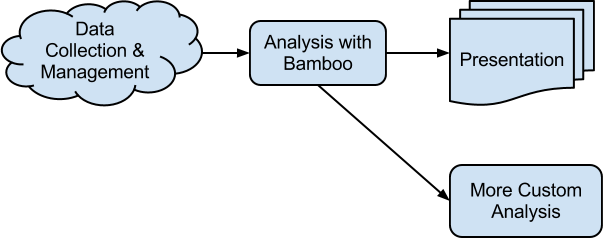
\includegraphics[width=3in]{figures/bamboo_flow}
\caption{Systematizing data collection and reporting with \textbf{bamboo}.}
\label{fig:flow}
\end{figure}

\textbf{bamboo} sits between data collection and reporting, as shown in Fig.
\ref{fig:flow}.
\textbf{bamboo}'s core functionality allows
practitioners to:
\begin{enumerate}
\item store, update, and merge datasets,
\item build algebraic calculations and aggregations, and
\item generate summary statistics: means, counts, etc.
\end{enumerate}
This exposes the split-apply-combine strategy of data analysis
\cite{wickham} through a web service.
The dynamic statistical analysis within \textbf{bamboo} allow practitioners to easily build
dashboards, maps, and tables.  These reporting tools will automatically update as new data
arrives.

Generalizability is a fundamental principle of the design: \textbf{bamboo} accepts any
CSV file and provides users with complete control over their calculations.
Updates can be submitted to \textbf{bamboo}'s application programming interface (API) using
JavaScript Object Notation (JSON) web requests, making it
simple to bring together data from a variety of sources.
These updates are propagated through the system ensuring that any aggregations
or merged datasets are synchronized with the most recent data, as depicted in Fig. \ref{fig:updates}.
To simplify updates, we have integrated \textbf{bamboo} with formhub, the mobile data collection platform,
such that updates to formhub can be automatically passed onto \textbf{bamboo}.
\textbf{bamboo} could be similarly integrated with ODK Aggregate and other data
collection platforms.

To encourage community use and development we have made the code open source and
structured it to be easily extendable. The \textbf{bamboo} web service uses
Representational State Transfer (REST)
conventions and we have written client libraries in Python and JavaScript that
connect to it.  For numerical computation \textbf{bamboo} uses pandas, a
Python library for high-performance statistical data analysis \cite{mckinney}.

\begin{figure}
\centering
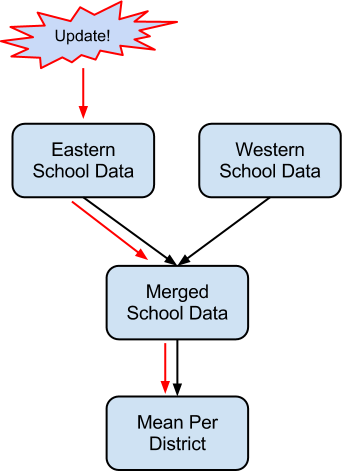
\includegraphics[width=3.5in]{figures/update_flow}
\caption{Red arrows show an update propagating to all downstream merged datasets and aggregations.  Black arrows show structural dependencies created by the client.}
\label{fig:updates}
\end{figure}

\section{Case Study}

During a large-scale data collection project in Nigeria, in which over 200,000 individual
surveys were conducted, researchers used
\textbf{bamboo} to monitor progress.
Specifically, as a public water facilities survey was conducted across the country
\textbf{bamboo} summarized the amount of data collected per state.
This provided data collection monitors with the tools they needed to identify states in which data coverage was lower than expected.

In addition, \textbf{bamboo} allowed researchers to conduct exploratory monitoring of this
dataset using complex metrics.  Fig. \ref{fig:summary} shows the number of waterpoints surveyed per 1000
people.  \textbf{bamboo} analyzed the raw survey data and created the summary
which powers this chart, ensuring that it
was up-to-date as additional data was collected.

\begin{figure}
\centering
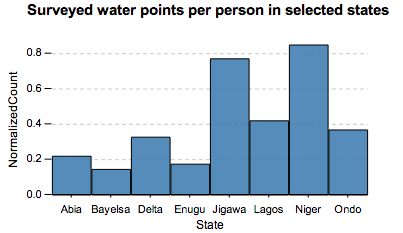
\includegraphics[width=3.5in]{figures/summary.png}
\caption{After merging datasets, the normalization formula required one API
    call. Thereafter, the same URL provides updated real-time data to create the graph above.}
\label{fig:summary}
\end{figure}

%\section{Discussion}

%Fig. \ref{fig:berg} shows a truncated version of a Community Health Worker 30 day performance monitoring table used in the ChildCount+ system \cite{berg}.  The ability to create and review this information was a crucial component of a larger system for improving the registration of children and ultimately health interventions, such as immunizations and monitoring risk factors.
%
%By connecting the ChildCount+ data collection infrastructure to Bamboo, practitioners are provided with the statistical analysis needed to build this table in \emph{real-time} as more data arrives.  Requiring only a minimal amount of effort and expertise, what were formerly static reports or charts can become dynamic monitor tools.
%
%\begin{figure}
%\centering
%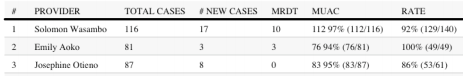
\includegraphics[width=3.5in]{figures/berg_table}
%\caption{A Community Health Worker 30 day performance monitoring table\cite{berg}.}
%\label{fig:berg}
%\end{figure}

\section{Future Work}
In future work we will focus on providing additional analysis relevant to
development work and methods to define and share this analysis.
We will add analysis tools to encompass more
real-world data processing tasks, such as Levenshtein distance, nearest
neighbors calculations, time series analysis, and spatial analysis.
From our field experience, we see the potential for a predefined library of common analysis techniques to reduce
efforts duplicated across domains.
Within certain domains we plan to offer ``calculation libraries'',
which codify common metrics for that domain.  For example, health researchers could
create a set of maternal health indicators once and then apply these same
indicators across all of their datasets.

\section{Conclusions}
\textbf{bamboo} allows users without programming expertise to perform real-time
data analysis.
We envision immediate application in the development context, making performance
monitoring \cite{berg} and real-time outlier detection within categorical data \cite{dimagi} much easier to implement. 
\textbf{bamboo} systematizes the process of creating indicators for domain specific datasets thereby reducing the time between collection and analysis, as well as the time between analysis and reporting.

%\end{document}  % This is where a 'short' article might terminate

%
% The following two commands are all you need in the
% initial runs of your .tex file to
% produce the bibliography for the citations in your paper.
\bibliographystyle{abbrv}
\small{
\bibliography{acm_dev2013_mrg}  % sigproc.bib is the name of the Bibliography in this case
}
% You must have a proper ".bib" file
%  and remember to run:
% latex bibtex latex latex
% to resolve all references
%
% ACM needs 'a single self-contained file'!
%
%APPENDICES are optional
%\balancecolumns

\balancecolumns
% That's all folks!
\end{document}
